\documentclass[tikz,border=4pt]{standalone}
\usepackage{tikz}
\usetikzlibrary{positioning}

\begin{document}
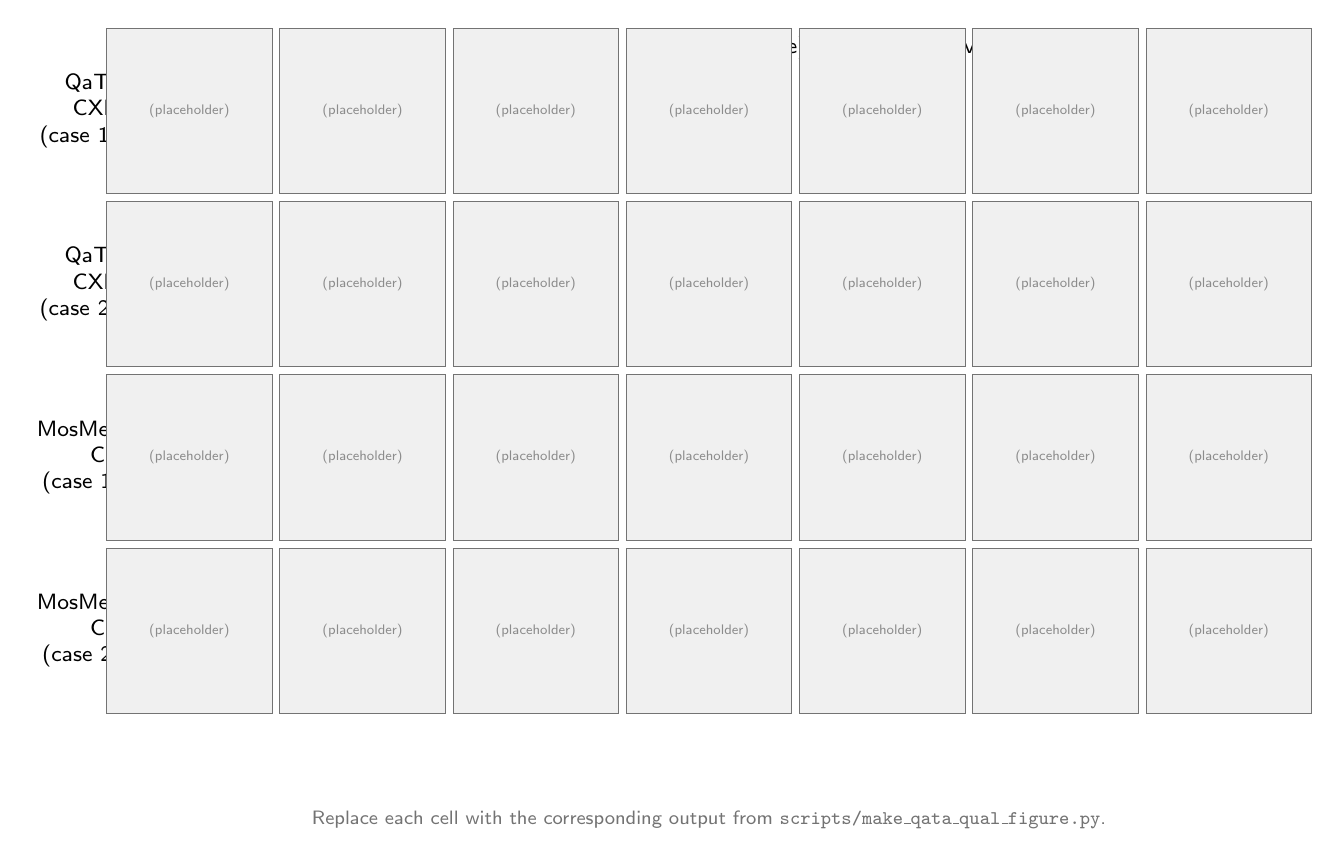
\begin{tikzpicture}[
  font=\sffamily\small,
  cell/.style={rectangle, draw=black!55, line width=0.3pt,
               minimum width=21mm, minimum height=21mm, inner sep=0pt,
               fill=black!6, align=center},
  hdr/.style={font=\sffamily\footnotesize},
  rowlabel/.style={font=\sffamily\footnotesize, align=right}
]
% ---- column headers ----
\def\cols{{"(a) Input","(b) GT","(c) U-Net","(d) LViT-T","(e) MedCLIP-SAMv2","(f) FMISeg","(g) Ours"}}
\foreach \i in {0,...,6} {
  \pgfmathsetmacro\xc{\i*22}
  \pgfmathparse{\cols[\i]}\let\lbl\pgfmathresult
  \node[hdr] at (\xc mm, 0) {\lbl};
}

% ---- 4 rows of 7 cells ----
\def\rowlabels{{"QaTa\\CXR\\(case 1)","QaTa\\CXR\\(case 2)","MosMed\\CT\\(case 1)","MosMed\\CT\\(case 2)"}}
\foreach \r in {0,...,3} {
  \pgfmathsetmacro\yc{-\r*22 - 8}
  \pgfmathparse{\rowlabels[\r]}\let\rl\pgfmathresult
  \node[rowlabel] at (-14mm, \yc mm) {\rl};
  \foreach \c in {0,...,6} {
    \pgfmathsetmacro\xc{\c*22}
    \node[cell] at (\xc mm, \yc mm) {\tiny\color{black!45} (placeholder)};
  }
}

% caption-like note below
\node[font=\sffamily\scriptsize, color=black!55, align=center]
  at (66mm, -98mm)
  {Replace each cell with the corresponding output from
   \texttt{scripts/make\_qata\_qual\_figure.py}.};

\end{tikzpicture}
\end{document}
